\chapter{}

\section{Implementación}

\subsection{Programa}
A la hora de implementar el programa una variable importante es la facilidad con la que se puede trabajar con la API para bots de Telegram. Debido a ello, y como quería que el proyecto fuera el desarrollo de pradobot y no de un programa para trabajar con la API de Telegram, opté por el uso de una librería que facilitara la tarea. En el momento de empezar la implementación las más populares eran:


\begin{itemize}
\item Para NodeJS: \url{https://github.com/yagop/node-telegram-bot-api}
\item Para Python: \url{https://github.com/python-telegram-bot/python-telegram-bot}
\item Para Golang: \url{https://github.com/go-telegram-bot-api/telegram-bot-api}
\item Java: \url{https://github.com/rubenlagus/TelegramBots}
\item Ruby: \url{https://github.com/atipugin/telegram-bot-ruby}
\end{itemize}

Teniendo conocimiento de Ruby y habiendo probado en alguna asignatura el correcto funcionamiento de la librería de Ruby, decidí usarla. Esta librería te permite hacer uso de los métodos de la API para bots de Telegram con un formato \textit{camel\_case} es decir las palábras de los métodos en minúscula y separadas por una barra baja. Por lo demás acepta los mismos parámetros:



\begin{figure}[H] %con el [H] le obligamos a situar aquí la figura
\centering
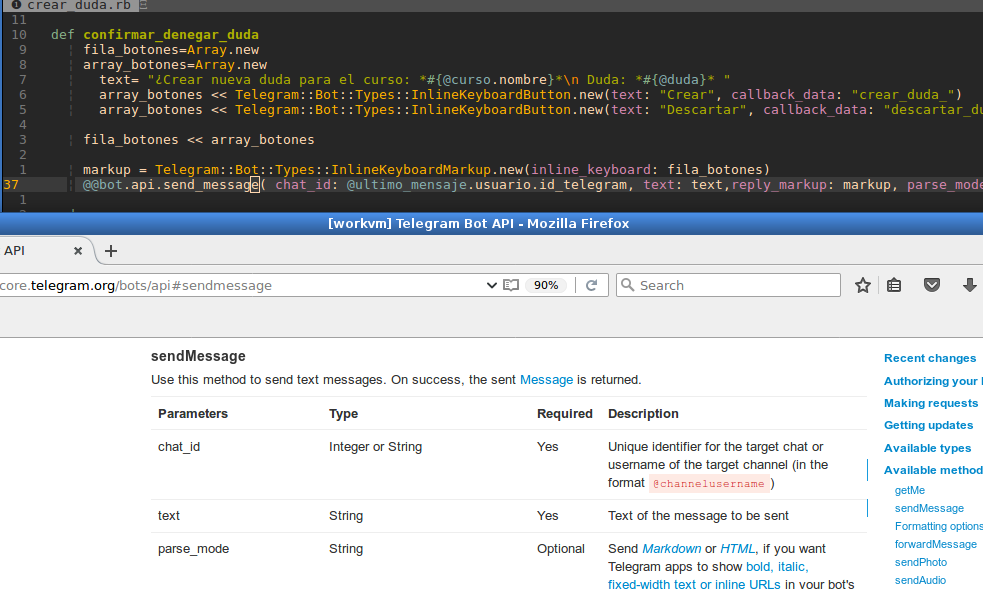
\includegraphics[scale=0.42]{imagenes/random/Screenshot_2017-08-27_08-16-42.png}  %el parámetro scale permite agrandar o achicar la imagen. En el nombre de archivo puede especificar directorios

\caption{Uso del método SendMessage por parte del bot }\label{figura531}
\end{figure}
El único inconveniente que tiene es que solamente puede haber una instancia del cliente que recibe mensajes. Esto es debido a que para que un bot de Telegram reciba los mensajes que le llegan tiene dos alternativas \textit{long polling} y \textit{Webhook} :
\begin{itemize}
\item \textit{Long polling}: El bot periódicamente llama a los servidores de Telegram utilizando un método que devuelve los 100 primeros mensajes  sin contestar que tiene el bot. Más lento pero mucho más facil de utilizar.
\item \textit{Webhook}: Hace falta implementar un servidor con una IP pública o un nombre de dominio e indicarle a Telegram que cuando se le manda un mensaje al bot éste lo redirija a este servidor. Rápido pero más complicado de montar.
\end{itemize}

El bot ha sido implementado haciendo uso de long polling y la implementación que realiza la librería utilizada  solamente deja que haya una instancia del bot \textbf{escuchando}:


\begin{figure}[H] %con el [H] le obligamos a situar aquí la figura
\centering
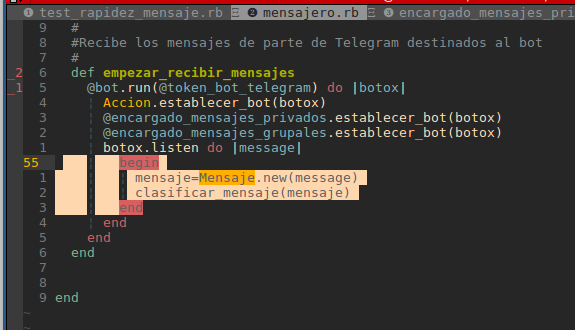
\includegraphics[scale=0.7]{imagenes/random/Screenshot_2017-08-27_11-49-39.png}  %el parámetro scale permite agrandar o achicar la imagen. En el nombre de archivo puede especificar directorios

\caption{ }\label{figura531}
\end{figure}

Lo cual a efectos prácticos implica que solamente puede haber un único :

\begin{lstlisting}

      botox.listen do |message|
        begin
          .....
        end
      end
 
\end{lstlisting}



\par 

 Una vez tienes el programa escrito en ruby que es capaz de obtener los mensajes que se le envían al bot por Telegram y de interactuar con los usuarios quedan dos partes más: la base de datos y la instancia de Moodle. 
 
 \subsubsection{Git-Github}
 
  Con la intención de que la construcción de la aplicación fuera lo más transparente posible y de dar la posibilidad de que otras personas pudieran contribuir a ella, se ha he hecho uso de la plataforma de desarrollo colaborativo Github y del sistema de control de versiones Git durante todo el proceso de implementación de la aplicación. 
  
  Github permite, entre otras cosas, ver los cambios realizados en el código desde el primer momento, la creación de \textit{issues} que pueden ser utilizados para indicar algún fallo en la aplicación y junto con git permite tener varias versiones del código.
  
 Todo el código del programa se puede encontrar en \url{https://github.com/LuisGi93/pradobot}.


\subsection{Base de datos}

Como base de datos he utilizado PostgreSQL principalmente porque es \textit{opensource}, fácil de instalar y no he visto en ningún sitio que tenga diferencias de rendimiento significativas comparada con otras bases de datos importantes. Aún así debido al uso de una librería de ruby llamada \href{https://github.com/jeremyevans/sequel}{Sequel}, que hace de adaptador entre la aplicación y la base de datos, se podría utilizar cualquier otra base de datos.

Sequel hace uso de ORM para la comunicación con la base de datos. También ofrece una capa de  abstracción entre aplicación y el manejo de todo lo relacionado con la interacción sobre la base de datos. Algunas de las carácteristicas relevantes para su uso:

\begin{itemize}
\item Ofrece configurar el número de conexiones disponibles para acceder a la base de datos.\cite{sequel1}
\item Una instancia de la \enquote*{conexión} con la base de datos hace uso de manera transparente para el programador de múltiples hebras para utilizar las conexiones disponibles de la base de datos. Lo cual implica que una misma variable  puede ser usada a lo largo del programa para realizar consultas con la base de dato sin que una consulta paralice al programa ya que serán ejecutadas por diferentes hebras.
\item Las conexiones descritas en el primer punto se levantan en el momento en que se lanza la primera consulta \cite{sequel2} quedando latentes a la espera de ser usadas por las siguientes consultas. Es decir no se abre una sesión con la base de datos, se realiza la consulta y se cierra la conexión, sino que está diseñado para que una misma conexión sea usada por diferentes consultas. Una correcta configuración del número de conexiones que se quiere que se tengan disponibles para la base de datos y del número de hebras a usar sobre esas conexiones es importante para un uso óptimo de la base de datos. Pradobot es un prototipo, y si se quisiera utilizar en un ambiente \enquote*{real}, esta sería una de las cosas que habría que mirar con lupa.
\item La abstracción que te ofrece el uso de ORM simplifica mucho el trabajar con la base de datos.
\end{itemize}

\subsection{Moodle}

Durante el desarrollo del programa se ha utilizado la versión 3.2.1 de Moodle. Aunque también se ha probado con la versión 3.0.10 y sea posiblemente la versión mínima soportada por el programa ya que las anteriores versiones no tienen algunas de las funciones de la API de Moodle utilizadas por el programa.


\subsection{Despliegue}

Para facilitar la instalación de la aplicación incluimos un fichero \enquote*{Vagrantfile} que permite la creación de una máquina virtual con Ubuntu 14.04 en Amazon AWS con pradobot y todas sus dependencias instaladas en ella. El contenido del Vagrantfile es el siguiente:

Para poder utilizar el Vagrantfile necesitamos tres programas: 

\begin{enumerate}
\item Instalar programa vagrant para nuestra distribución.
\item aws-cli: programa que nos permite conectarnos con nuestra cuenta en amazon aws y que genera credenciales para Vagrantfile (pip install awscli) .
\item Plugin aws para vagrant (vagrant plugin install vagrant-aws)
\end{enumerate}

El contenido de un Vagrantfile es similar al siguiente:
\begin{lstlisting}

Vagrant.configure("2") do |config|
  config.vm.box = "dummy"

  config.vm.define "pradobot-aws" do |host|
    host.vm.hostname = "pradobot-aws"
  end
  config.vm.provider :aws do |aws, override|
    aws.access_key_id = "xxx"
    aws.secret_access_key = "xxx"
    aws.session_token = "xxx"
    aws.keypair_name = "pradobotllave"
    aws.region= "us-west-2"
    aws.security_groups = "migruposeguro"
    aws.instance_type= 't2.micro'
   
    aws.ami = "ami-d57dcfb5"

    override.ssh.username = "ubuntu"
    override.ssh.private_key_path = "pradobotllave.pem"
  end
  
    config.vm.provision :ansible do |ansible|
	ansible.playbook = "pradobot.yml"
	ansible.force_remote_user= true
  end
end
 
\end{lstlisting}

El Vagrantfile cuenta con los siguientes elementos:
\begin{itemize}
\item \textbf{aws.secret\_access\_key}, \textbf{aws.session\_token}: Claves efímeras que nos autorizan para crear máquinas virtuales en nuestra cuenta durante 48 horas. Generadas utilizando aws-cli:

\begin{figure}[H] %con el [H] le obligamos a situar aquí la figura
\centering
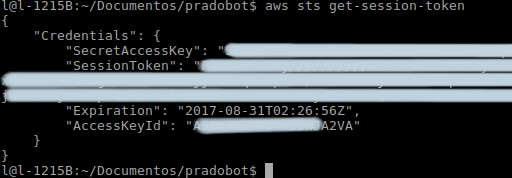
\includegraphics[scale=0.6]{imagenes/random/1234sts.png}  %el parámetro scale permite agrandar o achicar la imagen. En el nombre de archivo puede especificar directorios

\caption{Utilizando aws-cli para generar claves efímeras para el despliegue}\label{figura90}

\end{figure}
\item \textbf{aws.keypair\_name}: Generada utilizando:
\begin{lstlisting}
 aws ec2 create-key-pair --key-name pradobotllave --query 'KeyMaterial' --output text > pradobotllave.pem
\end{lstlisting}
\item \textbf{aws.security\_groups}: Grupo de seguridad en Amazon AWS en  podemos especificar que puertos de entrada/salida están habilitados en la máquina virtual y que IPs aceptamos.
\item \textbf{aws.region},\textbf{aws-instance\_type},\textbf{aws.ami}: Especifican la región, las características del servidor donde se ejecuta la máquina virtual y el sistema operativo.
\item Por último \textbf{config.vm.provision} especifica que queremos usar Ansible para aprovisionar la máquina virtual:
\begin{itemize}
\item \textbf{ansible.playbook}: script que utilizará ansible para aprovisonar la máquina virtual.
\end{itemize}
\end{itemize}

\subsection{Aprivisionamiento}

El aprovisionamiento de la máquina virtual creada por vagrant se hace utilizando el programa Ansible. Ansible hace uso de ssh y de un tipo de archivos llamados \enquote*{playbooks} en las cuales se especifican las órdenes necesarias para el aprovisonamiento de la máquina virtual. El playbook utilizado por pradobot es el siguiente:
\begin{lstlisting}

---
---
- hosts: all
  user: ubuntu
  sudo: yes    
  roles:
    - { role: rvm_io.ruby,
        tags: ruby,
        rvm1_rubies: ['ruby-2.3.1'],
        rvm1_user: 'ubuntu',
        become: true
      }
      
  tasks:       


#Por alguna razon instala todos los paquetes menos libpq-dev

  -  name: Instalamos  paquetes necesarios
     become: true
     action: >
      {{ ansible_pkg_mgr }} name= {{ item }}  state=installed update_cache=yes
     with_items:
      - build-essential
      - ruby-dev
      - libpq-dev
      - ruby
      - git
      - libgdbm-dev
      - libncurses5-dev
      - automake
      - libtool
      - bison
      - libffi-dev
     
  -  name: instalamos git
     apt:
       name: git
       state: present

  -  name: instalamos libpq-dev
     apt:
       name: libpq-dev
       state: present

  -  name: clonamos repo de la web
     become: true  
     become_user: ubuntu
     shell: git clone  https://github.com/LuisGi93/pradobot.git
     args:
       creates: pradobot
       executable: /bin/bash

  -  name: Instalamos el proyecto
     become: true  
     become_user: ubuntu 
     shell: source ~/.rvm/scripts/rvm && bundle install 
     args:
       chdir: pradobot
       executable: /bin/bash
     
      -  name: Creamos las tablas de la base de datos
     become: true  
     become_user: ubuntu 
     shell: source ~/.rvm/scripts/rvm && export URL_DATABASE_TRAVIS="" &&  ruby config/primer_inicio_aplicacion.rb
     args:
       chdir: pradobot
       executable: /bin/bash
\end{lstlisting}

En el cual podemos distinguir las siguientes partes relevantes:
\begin{itemize}

\item \textbf{hosts}, \textbf{user}: Indicamos el nombre de la máquina a la que se va a conectar Ansible utilizando ssh.
\item \textbf{user}: nombre del usuario con el cual se inicia sesión en dicha máquina utilizan ssh.
\item \textbf{sudo}: Indicamos si se va utilizar sudo o no.
\item \textbf{roles}:  Indicamos que para ejecutarse este playbook se necesitan una serie de archivos, en este caso rvm que explico más abajo para que sirve.
\item \textbf{tasks}: Tareas a ejecutar por Ansible secuencialmente, algunos de los elementos que pueden tener son:
\begin{itemize}
\item \textbf{name}: nombre descriptivo.
\item \textbf{become}: implica el uso de sudo.
\item \textbf{become\_user}: implica el usuario a utilizar.
\item \textbf{shell}: el comando se tiene que ejecutar en una shell.
\item \textbf{apt}: requiere el uso del administrador de paquetes.
\end{itemize}

\end{itemize}

El script en primer lugar instala los paquetes necesarios, tras lo cual clona el proyecto desde github creando el directorio pradobot y procede a instalar las dependencias de pradobot utilizando RVM y Bundler.\\
RVM es un programa que permite la ejecución de otro programa escrito en ruby en el entorno de ruby deseado, en mi caso pradobot necesita la versión 2.3.1 de ruby que no se encuentra en los repositorios de Ubuntu. Bundler automatiza la instalación de las librerías que necesita una aplicación de ruby para lo cual hace uso de un archivo llamado Gemfile:
\begin{lstlisting}[language=Ruby]

source "https://rubygems.org"
gem 'sequel'
gem 'pg'
gem 'rake'
gem 'rspec'
gem 'telegram-bot-ruby'
gem 'json'
gem 'rufus-scheduler'
gem 'activesupport'
gem 'daemons'
gem 'typhoeus'
group :test do
  gem 'rake'
end
\end{lstlisting}
En el se especifican las librerías a obtener, su versión si se quiere y de donde obtenerlas. Por último inicia la ejecución de pradobot.

\subsection{Control ejecución}

Una vez hemos creado la máquina con Vagrant y haberla aprovisionado utilizando Ansible, tenemos que poder controlar el inicio y fin de ejecución de la aplicación de manera automática. Para ello vamos a utilizar una herramienta llamada Capistrano. Capistrano permite la ejecución de comandos remotos a través de ssh. En primer lugar lo instalamos haciendo \texttt{gem install capistrano} tras lo cual ejecutamos la orden \texttt{cap install} en el directorio de nuestro proyecto. Esto provocará la generación de una serie de archivos. Buscamos \enquote*{config/deploy.rb} y le añadimos información para la autenticación via ssh:
\begin{lstlisting}[language=Ruby]

set :ssh_options, {
  forward_agent: true,
  auth_methods: ["publickey"],
  keys: ["path_a_llave_pem/pradobotllave.pem"]
}

\end{lstlisting}

En Capistrano se definen "tareas" donde defines que es lo que quieres que haga capistrano. Para establecer la tarea creamos un fichero en lib/capistrano/tasks acabado en .rake y en el defino la siguiente tarea:


\begin{lstlisting}[language=Ruby]

require "resolv-replace.rb"

role :yoquese, "yoquese"


namespace :pradobot do
  desc "Iniciamos la aplicacion"

  task :daemon_start do
	on "ubuntu@ip.us-west-2.compute.amazonaws.com" do
		execute  'source ~/.rvm/scripts/rvm && export TOKEN_BOT_MOODLE="" && export MOODLE_HOST="" && export TOKEN_BOT="" && export URL_DATABASE_TRAVIS="" && nohup ruby pradobot/bin/run.rb && true & '
	end
  end
  
  desc "Paramos la aplicacion"  
  task :daemon_stop do
	on "ubuntu@ip.us-west-2.compute.amazonaws.com" do
		execute  'pkill ruby'
	end
  end
end

\end{lstlisting}

Con lo cual podemos ejecutar el comando \texttt{cap production pradobot:daemon\_start} para iniciar su ejecución y pararlo utilizando \texttt{cap production pradobot:daemon\_stop}. \par Para el inicio de la ejecución se hace uso del comando nohup, que desliga a un proceso de la terminal de tal forma que cuando se lanza el programa en segundo plano (\texttt{ruby pradobot/bin/run.rb \&\& true \&}) su ejecución no termina al finalizar la ejecución de la orden por ssh. 

\subsection{Tests}


Los tests se han implementado utilizando Rake. Rake es una herramienta que permite entre otras cosas ejecutar tests de ruby para lo cual necesita disponer de un archivo llamado Rakefile en el cual se le indica dónde puede encontrar los tests y qué pasos hay que dar para ejecutarlos. El Rakefile de pradobot es el siguiente:

\begin{lstlisting}[language=Ruby]

require 'rake/testtask'
require 'rspec/core/rake_task'
require_relative 'config/crear_tablas_bd'
require 'sequel'



namespace :tasks do
  namespace :db do
    namespace :test do

      desc "Creamos base de datos test"
      task :crear  do
        db=Sequel.connect(ENV['URL_DATABASE'])
        begin
          db.run "CREATE DATABASE bd_prueba"
        rescue Sequel::Error
          db.run "DROP DATABASE bd_prueba"
          db.run "CREATE DATABASE bd_prueba"
        end
        db.disconnect
        db=Sequel.connect(ENV['URL_DATABASE']+'/bd_prueba')
        crear_tablas(db)
        db.disconnect
        ENV['URL_DATABASE_ORIGINAL']=ENV['URL_DATABASE']
        ENV['URL_DATABASE']=ENV['URL_DATABASE_PRUEBA']
      end

      RSpec::Core::RakeTask.new(:tests_bd) do |t|
          t.pattern = Dir.glob('test/test_*.rb')

          t.rspec_opts = '--format documentation'
      end

      desc "Borramos la base de datos"
      task :destruir  do
        ENV['URL_DATABASE']=ENV['URL_DATABASE_ORIGINAL']
        db=Sequel.connect(ENV['URL_DATABASE'])
        db.run "DROP DATABASE bd_prueba"
        db.disconnect
      end

    end

  end




end


desc "Ejecutamos los test sobre la base de datos"
task :default => ['tasks:db:test:crear', 'tasks:db:test:tests_bd', 'tasks:db:test:destruir' ]
\end{lstlisting}

En él se especifican las tareas que tiene que ejecutar Rake:
\begin{itemize}
\item \textbf{task :default}: Es la tarea que se llama por defecto subdividida en tres tareas:
\begin{enumerate}
\item \textbf{tasks:db:test:crear} : Crea una base de datos de prueba e insertamos las tablas que componen la aplicación.
\item \textbf{tasks:db:test:tests\_bd} : Indica a Rake que ejecute como tests todos los archivos contenidos en la carpeta test/ y que empiecen por test\_.
\item \textbf{tasks:db:test:destruir}: Destruye la base de datos creada en el paso 1.
\end{enumerate}

\end{itemize}

Para la realización de los tests he hecho uso de la librería RSpec que proporciona las herramientas necesarias para la realización de los mocks y los stubs. Un ejemplo de test puede ser:

\begin{lstlisting}[language=Ruby]

describe CrearDuda do
  before(:each) do
    @stub_bot = double('bot')

    Accion.establecer_bot(@stub_bot)

    allow(@stub_mensaje).to receive_message_chain(:usuario, :id_telegram) { 66 }

    @stub_curso = double('curso')
    allow(@stub_curso).to receive(:nombre) { 'nombre del curso' }
    allow(@stub_curso).to receive(:id_moodle) { 5 }
    stub_padre = double('accion_padre')
    allow(stub_padre).to receive(:cambiar_curso)
    allow(stub_padre).to receive(:cambiar_curso_parientes)
    allow(stub_padre).to receive(:curso) { @stub_curso }
    @accion = MenuDudas.new(stub_padre)
    @accion.cambiar_curso(@stub_curso)
  end

  it 'Cuando recibe el primer mensaje muestra mensaje explicativo de que realiza' do
    allow(@stub_mensaje).to receive(:datos_mensaje) { 'Nueva duda' }
    expect(@stub_bot).to receive_message_chain(:api, :send_message) { |arg1|
      arg1.keys.should_not include(:reply_markup)
      arg1[:text].should eq("Escriba a continuaci\otilden la duda que desea crear relacionada con *nombre del curso*:\n")
    }
    @accion.recibir_mensaje(@stub_mensaje)
  end

  it 'Debe mandar mensaje que incluya el texto de la duda y el curso con opciones para confirmar la creaci\otilden de la duda' do
    allow(@stub_mensaje).to receive(:datos_mensaje) { 'Nueva duda' }

    allow(@stub_bot).to receive_messag_chain(:api, :send_message)
    @accion.recibir_mensaje(@stub_mensaje)

    allow(@stub_mensaje).to receive(:datos_mensaje) { 'Contenido nueva duda' }

    expect(@stub_bot).to receive_message_chain(:api, :send_message) { |arg1|
      arg1.keys.should include(:chat_id, :text, :reply_markup)
      arg1[:text].should include('nombre del curso')
      arg1[:text].should include('Contenido nueva duda')
      arg1[:reply_markup].should be_instance_of(Telegram::Bot::Types::InlineKeyboardMarkup)
    }
    @accion.recibir_mensaje(@stub_mensaje)
  end
  
   .....
end

\end{lstlisting}

Al principio se define stub\_bot que actúa a la vez como mock y stub para, a continuación, especificarse los métodos que tiene que aceptar mediante la orden \texttt{allow(stub).to receive(nombre método)[ datos respuesta ]}.
\par
En esta fragmento de código podemos encontrar dos tests que vienen compredidos entre el \texttt{it .. do} y el \texttt{end} que lo cierra. En los dos tests mostrados  se definen mediante la orden \texttt{expect(stub).to receive(nombre método)[  argumentos ]} las expectativas del test.
\begin{itemize}
 \item En el primero el objeto stub\_bot espera que se llame al método 
 \texttt{stub\_bot.api.send\_message} que se le pase como argumento un objetivo tipo hash que entre sus llaves no tenga una llamada \texttt{:reply\_markup} y sí una llave llamada \texttt{text} que tenga el valor de \texttt{"Escriba a continuación la duda que desea crear relacionada con *nombre del curso*:"}. 
 \item El segundo test es parecido solo que ahora se observa el comportamiento de la clase cuando ha recibido su segundo mensaje y se comprueba qué le manda al bot como respuesta de este segundo mensaje.
 \end{itemize}
 \par
 
 Por último para ver la cobertura sobre el código del programa que tienen nuestros tests y comprobar en qué puntos de la aplicación faltan pruebas unitarias por realizar se ha hecho de una librería llamada \textbf{SimpleCov}.
